\section{Vegetation}

Vegetation is core to rural landscapes. The species present along with their associated densities create a relationship between ecosystems and areas on earth on which resources are adequate. To ensure realism in virtual rural worlds, much emphasize must be put on efficiently modelling these underlying ecosystems.\\

This section will review different methods to generate suitable vegetation for virtual worlds. These methods can be split into three main categories: \textit{Explicit Instancing, Probabilistic Instancing} and \textit{Plant Growth Modelling}.\\

\textit{Explicit Instancing} require explicit user-input to directly or indirectly pinpoint exact locations for individual plant instances.\\

\textit{Probabilistic Instancing} methods use statistical models to generate suitable vegetation.\\ 

\textit{Simulators} attempt to algorithmically reproduce plants battling for available resources.\\

\subsection{Explicit Instancing} \label{Explicit Instancing}
Explicit instancing methods require input from the user to explicitly outline the location of individual plant instances. \\

Arnaud et al. \cite{Emilien} permit users to insert individual plants manually by simply clicking the appropriate location on the terrain. To overcome the tedious task of manually placing individual plant instances on large terrains, the system is able to analyse existing distributions for reproduction. For example, to generate a large forest, the user is only required to generate a small subsection which can then be used to reproduce it on any scale (figure \ref{Explicit instancing as input examplars}) \\

\begin{figure}[h]
  \centering
	\label{Explicit instancing as input examplars}
	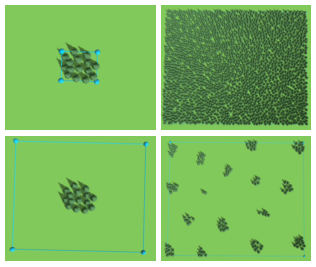
\includegraphics[natwidth=316,natheight=267]{worldbrush_forrest_reproduction.png}
	\caption{Using explicit instancing as input examplars for reproduction \cite{Emilien}}
\end{figure}

Similarly, Deussen et al. \cite{Deussen1998} allow users to use grayscale raster images as input to specify terrain vegetation. The location of individual plants is determined by pixel location whereas plant properties are correlated to pixel intensity.\\

During their work focused on improving the realism of roadside landscapes, Andujar et al. ~\cite{Andujar2014} use orthophotos as input to determine the location and properties of individual plants. Unlike ordinary aerial photographs, aerial orthophotos use normalisation techniques to take into account terrain relief and camera tilt to produce the image. The result is an image with uniform scale throughout, which, similarly to a map, can be used to accurately measure distances between points. Here, the orthophotos are analysed to determine the center point of individual plants.\\

\begin{figure}[!htb]
  \centering
	\label{Reconstructed roadside vegetation using orthophotos}
	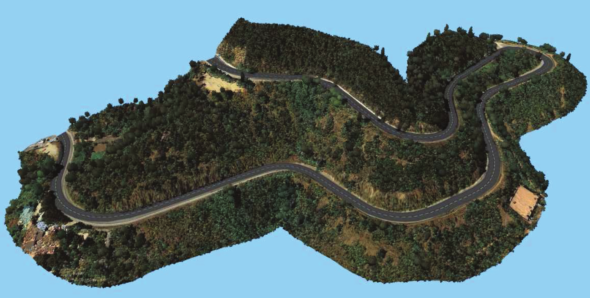
\includegraphics[width=\textwidth]{reconstructed_roadside_vegetation.png}
	\caption{Reconstructed roadside vegetation using orthophotos ~\cite{Andujar2014}}
\end{figure}

Explicit instancing methods provide extensive user control over the resulting vegetation. However, although some automation is provided, it is often limited. It does take some of the burden off the artist but generating large realistic virtual worlds with varying plant species will still be a lengthy process. \\

\subsection{Probabilistic Instancing} \label{Probabilistic Instancing}

Probabilistic instancing methods use statistical models in an attempt to produce adequate vegetation. These methods can be further split into two sub-categories which are discussed in further detail below: \textit{Radial Distribution Analysis} and \textit{Predefined Ecosystems}.\\

\subsubsection{RADIAL DISTRIBUTION ANALYSIS}
Work by Emilien et al. \cite{Emilien}, Boudon et al. \cite{Boudon2007} and Lane et al. \cite{Lane2002} use radial distribution analysis to convert to metric form the underlying plant distributions of input examplars. The data generated by the analysis stage can later be used to synthesise, at any scale, new point distributions which respect the characteristics of the input exemplar \cite{Oztireli2012}. \\
For example, by analysing the positions of individual plants in a small subset of a forest and using it as the input exemplar, it is possible to reproduce it at a much larger scale in order to model its full size counterpart.\\

\paragraph{Analysis}
Generating the analytical data involves measuring the distances between individual points of different categories from the input examplar. For plant distribution analysis, the points represent individual plant instances and the categories represent the different species.\\

Before performing the analysis, the following parameters need to be configured:
\begin{itemize}
\item \textbf{R\textsubscript{min}}: The minimum distance from which point distances need to be analysed.\\
\item \textbf{R\textsubscript{max}}: The maximum distance after which point distances don't need to be analysed.\\
\item \textbf{Bin size}: When analysing the distances of given points, it is necessary to aggregate the points which reside at similar distances into bins. The bin size is the range represented by a single bin.\\
\end{itemize}

A core part of radial distribution analysis is generating pair correlation histograms for each category pair combination. A pair correlation histogram \textit{H\textsubscript{AB}} represents the variation in the distance between points of of category \textit{C\textsubscript{A}} and \textit{C\textsubscript{B}} ranging from \textit{R\textsubscript{min}} to \textit{R\textsubscript{max}} in \textit{bin size} increments (figure \ref{Pair Correlation Histograms}) \\

\begin{figure}[h]
  \centering
	\label{Pair Correlation Histograms}
	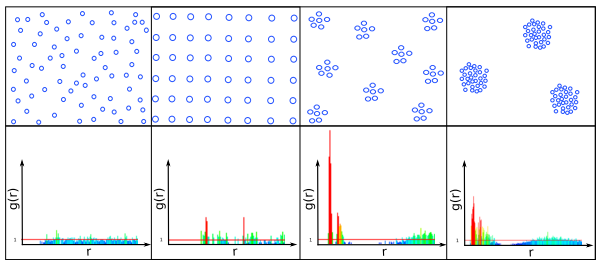
\includegraphics[width=\textwidth]{pair_correlation_histograms.png}
	\caption{Point distributions with associated pair correlation histogram \cite{Emilien2014}}
\end{figure}

To generate the pair correlation histogram \textit{H\textsubscript{AB}}, the algorithm iterates through each reference point of category \textit{C\textsubscript{A}} and, for each destination point of category \textit{C\textsubscript{B}} at a distance between \textit{R\textsubscript{min}} and \textit{R\textsubscript{max}}, increments the relevant bin in the histogram. In figure \ref{Radial distribution analysis}, for example, are being measured the points that lie within the annular shell of radius \textit{r} with bin size \textit{d\textsubscript{r}} (area \textit{d\textsubscript{A}}). 

\begin{figure}[h]
  \centering
	\label{Radial distribution analysis}
	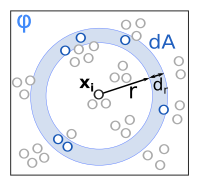
\includegraphics[natwidth=199,natheight=140]{radial_distribution_analysis.png}
	\caption{Radial distribution analysis}
\end{figure}

Because of their larger circumference, the coverage area of annular shells get larger as the distance bin being measured increases. In other words, \textit{A\textsubscript{r}} \textless \textit{A\textsubscript{r+1}} where \textit{A\textsubscript{r}} is the area covered by the annular shell starting at distance \textit{r}. A direct consequence of this is that annular shells at further distances will naturally be prone to containing more points. To counter for this, normalisation is performed based on annular shell area. \\

The radial distribution analysis function \textit{h\textsubscript{rdf}} is as follows:\\
\begin{center}	
$h_{rdf}(k) = \sum_{x_{i} \in X} \sum_{y_{j} \in Y \&  
kd_{r} \leq d(x_{i}, y_{j}) < (k+1)d_{r} } \frac{A}{d_{A}n_{x}n_{y}} $
\end{center}
Where:
\begin{itemize}
\item \textit{hrdf(k)} is the k-th value of the pair wise histogram.
\item \textit{X} are the points of category X (reference points).
\item \textit{Y} are the points of category Y (target points)    .
\item \textit{d\textsubscript{r}} is the annular shell width.
\item \textit{A} is the total analysed area.
\item \textit{n\textsubscript{x}} and \textit{n\textsubscript{y}} are the number of points of categories \textit{x} and \textit{y} respectively.
\item \textit{d\textsubscript{A}} is the area of the annular shell being analysed.
\end{itemize}

Conceptually, this formula calculates the variance from the average density of the target category at incremental distances from points of the reference category.\\

\paragraph{Reproduction}

In order to reproduce the distribution of the input exemplar, points are added iteratively whilst matching as closely as possible the corresponding pair correlation histogram data calculated during the analysis stage. Metropolis-Hastings sampling ~\cite{Hurtut2009} is the most common way to do this. It involves performing a fixed number of point birth-and-death perturbations. A change from the initial arrangement \textit{X} to the new arrangement \textit{X'} is accepted with probability \textit{R}, where:

\begin{center}
$ R = \frac{f(X')}{f(X}$
\end{center}
\textit{f(X)} is the probability density function (PDF) and is expressed as:\\

\begin{center}
$ f(X) = \prod_{C_{Y_{K}} \leq C_{X}} 
		 \prod_{x_{i} \in X}
		 \prod_{y_{i} \in Y_{k}} 
		 h_{X,Y_{k}}(d(x_{i},y_{j}))$
\end{center} 

Where:
\begin{itemize}
\item \textit{C\textsubscript{y}} and \textit{C\textsubscript{x}} represent categories \textit{Y} and \textit{X} respectively
\item \textit{X} are all points of category \textit{X}
\item \textit{Y} are all points of category \textit{Y}
\item h\textsubscript{X,Y\textsubscript{k}}(d(x\textsubscript{i}, y\textsubscript{j})) is the value retrieved from the pairwise histogram of categories \textit{X} and \textit{Y} given the distance between points \textit{x\textsubscript{i}} and \textit{y\textsubscript{i}}.
\end{itemize}
Intuitively, the PDF defines, given a set of points, the aggregate strength of the current distribution.\\

Because the PDF is a product, to calculate the PDF of a new layout \textit{X'} with appended/removed point \textit{P} it is only necessary to calculate the PDF of \textit{P}. As a consequence, reproduction can be performed very efficiently. In their work, Arnaud et al. ~\cite{Emilien} are able to perform analysis and reproduction in near real-time.\\

\subsubsection{PREDEFINED ECOSYSTEMS}

In their work, Hammes el al. \cite{Hammes2001} predefine ecosystems along with their preferred environment. This is defined in terms of:

\begin{itemize}
\item Elevation: All plant species have an upper limit after which temperature or oxygen levels are ill-suited.
\item Relative elevation: The local changes in height. Local minimums tend to be valleys and therefore wetter with less illumination. Local maximums, on the other hand, tend to me ridges which are dryer and much more exposed.
\item Slope: Gradient has a direct impact on the quality of the soil and therefore the plants which can grow. When slopes get steeper, plants tend to get much smaller as they struggle to get required nutrients from the soil.
\item Slope direction: This has a direct effect on sunlight exposure. Southern facing slopes in the northern hemisphere will have a greater exposure to the sun and vice-versa for the southern hemisphere.  
\end{itemize}

All these ecosystems are stored in a database and, when vegetation is to be placed on a given terrain, the most suitable ecosystems are chosen based on terrain properties mentioned above. See figure \ref{Vegetation generated using predefined ecosystems} for an example landscape generated using this technique.

\begin{figure}[h]
  \centering
	\label{Vegetation generated using predefined ecosystems}
	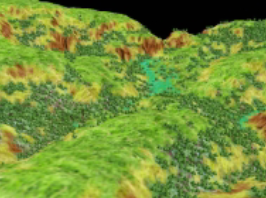
\includegraphics{predefined_ecosystems.png}
	\caption{Vegetation generated using predefined ecosystems \cite{Hammes2001}}
\end{figure}

\textit{Probabilistic Instancing} methods provide a good level of automation for artists to place vegetation on a given terrain. However, before these methods can be used, users must define input examplars. For the \textit{Radial Distribution Analysis} approach, this would be in the form of an input distribution. For the \textit{Predefined Ecosystems} approach, this would be a predefined ecosystem with its preferred environment. Realistic manual plotting, albeit in a much smaller area, is therefore still necessary.

\subsection{Simulators} \label{Simulators}

Another approach used to determine vegetation in a given environment is to simulate plants battling for available resources. This approach can be further split into two subcategories which are further examined below: \textit{Plant Growth Modelling} and \textit{Ecosystem Simulators}.\\

\subsubsection{PLANT GROWTH MODELLING}

These types of simulators attempt to reproduce algorithmically the laws of nature with such precision that they can be used in agronomical sciences and forestry to estimate and maximize crop yield. To do so, these type of simulators go into great detail to model the available resources. For example,  work by Soler et al. ~\cite{Soler2001} split single plants into geometrical organs with unique light transmittance and reflectance properties. By doing so, light propagation within the plant can be simulated in order to determine the aggregated photosynthetic potential. This work, along with work by Yan et al. ~\cite{Yan2004}, base their simulators on two vital and widely accepted laws of nature:

\begin{itemize}
\item \textit{Law of the sum of temperatures}: Plants grow in cycles which vary from days to years depending on the specie. The law of the sum of temperatures states that the frequency of these cycles is proportional to the sum of the daily average of the temperatures.
\item \textit{Law of the water use efficiency}: The amount of fresh matter fabricated by a plant is proportional to the water evaporation of the plant. This factor is called the water use efficiency. 
\end{itemize}

Water evaporates during photosynthesis as the plant exchanges water for carbon dioxide. Based on this and the law of water use efficiency outlined above, the amount of fresh matter produced for a given plant is directly correlated to the amount of photosynthesis performed. Using this, Soler et al. ~\cite{Soler2001} use the following formula to calculate the amount of fresh matter, \textit{Q\textsubscript{m}(t)}, created by a given plant at time \textit{t}:\\

\begin{center}	
\textit{$Q_{m}(t)$} = $\sum_{x=1}^{N(t)} \frac{E(x,t)}{\frac{r_{1}}{S(x,t)} + r_{2}} $
\end{center}
Where:
\begin{itemize}
\item \textit{E(x,t)} is the potential of matter production of the \textit{x}-th leaf at the \textit{t}-th cycle
\item \textit{r\textsubscript{1}} is the leaf blade resistance per unit area (specie dependant)
\item \textit{r\textsubscript{2}} is the average resistance of the leafs nerves and petiole (specie dependant)
\item \textit{S(x,t)} is the surface area of the \textit{x}-th leaf at the \textit{t}-th cycle
\end{itemize}
Intuitively, this formula calculates the total available fresh matter, \textit{$Q_{m}$}, that can be produced for an individual plant \textit{P} at a given time \textit{t} by calculating the photosynthesis potential of each individual leaf of \textit{P} given the current lighting.\\

Using this, the algorithm iterates through the following two-step growth cycles:
\begin{enumerate}
\item The lighting and therefore photosynthesis potential of each individual leaf of the plant is calculated. This is then used to calculate, using the formulae outlined above, the quantity of fresh matter produced.
\item The fresh matter is then distributed to different organs of the plant. To determine how to distribute the fresh matter, individual organs of the plant have associated strengths and, therefore, priority.
\end{enumerate}

By going into such detail, these simulators produce very realistic simulations of the evolution of plants. For example, to maximize growth potential, plants are able to grow in direction of the light source (figure \ref{Plant growing towards light source}).\\

Although the results are very realistic, going into such detail does make the simulations computationally expensive. In the work by Soler et al. ~\cite{Soler2001}, simulating 45 cycles for a single plant takes approximately 15 minutes. Because of this, only a small subset of plants can be simulated at once. \\
Also, to model the growth of these plants, topological data for each specie must be specified. Specifying this information can be a lengthy process as it often involves analysing various metrics of the plants growth cycles.

\begin{figure}[h]
  \centering
	  \label{Plant growing towards light source}
	    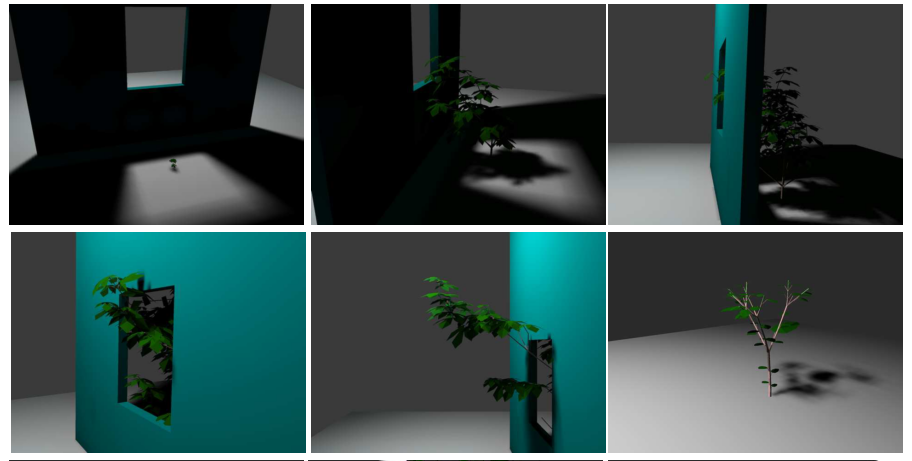
\includegraphics[width=\textwidth]{plant_growing_towards_light_source.png}
	\caption{Plant growing towards light source ~\cite{Soler2001} }
\end{figure}

\subsubsection{ECOSYSTEM SIMULATORS}

Ecosystem simulators use procedural methods to algorithmically reproduce the competition for resources that occurs in nature during plant growth. In nature, this competition is an extremely complex process and so reproducing it exactly would be infeasible. Instead, a simplified model of this ecological process is implemented. During these simulations, available resources fluctuate and each plants strength is continuously recalculated based on its associated properties. This strength directly affects the plants growth and chance of survival. \\
Plant properties include: age; vigor; shade tolerance; humidity requirement; temperature
requirements.\\
Modelled resources include: available illumination; available humidity; temperature; slope.

The aim of ecosystem simulators is to determine, given an initial state \textbf{\textit{S\textsubscript{t}}} of the system at time \textbf{\textit{t}} and a simulation time \textbf{\textit{n}}, the state \textbf{\textit{S\textsubscript{t+n}}}. \\
The state of the system represents individual plant instances with associated location and properties. \\

Lindenmayer systems, commonly referred to as L-systems, use formal grammar along with a set of production rules to iteratively create larger strings from a starting string called the axiom. Such systems are commonly used to model plants and plant growth ~\cite{Prusinkiewicz1990,Deussen2002,Boudon2012,Prusinkiewicz1993}. \\
An extension to the basic L-systems, referred to as open L-systems, adds communication grammar which permits the set of production rules to behave differently depending on predefined conditions ~\cite{Prusinkiewicz1996}.\\ 
By introduction multiset L-Systems, Lane et al. ~\cite{Lane2002} extend this further in to model an ecosystem simulator. The production rules for multiset L-systems work in two stages. The first, identical to basic L-Systems, produces a new string given an input string and production rule. The second, splits the resulting string into new sets using a predefined separation symbol. In their work, the different sets represent different plant instances, thus enabling new plants to spawn during the production steps. When building their L-System, Lane et al. ~\cite{Lane2002} focused on reproducing three important properties of nature. Each distinctly testable to determine the plausibility of the results:
\begin{itemize}
\item \textit{Self-thinning}: When plants grow, their resource requirements increase and, as a direct consequence, inter plant competition for resources increases. Eventually, the competition becomes too intense and resources too scarce leading to more vigorous plants starving smaller plants. At this point, self thinning begins and plant densities decrease.
\item \textit{Succession}: Given plant specie \textit{A} with a fast growth rate and specie \textit{B} with a slower growth rate but high shade tolerance. At first, the faster growing specie \textit{A} will dominate and flourish. With time, however, slower growing but shade tolerant specie \textit{B} will flourish and dominate.
\item \textit{Propagation}: Plants often propagate in clusters surrounding the seeding plant.
\end{itemize}

The L-System they implemented contained different production rules to represent the different properties of nature mentioned above. A single simulation and the corresponding output can be seen in figure ~\ref{Plant placement using an ecosystem simulator modelled by L-System}

\begin{figure}[h]
  \centering
    \label{Plant placement using an ecosystem simulator modelled by L-System}
    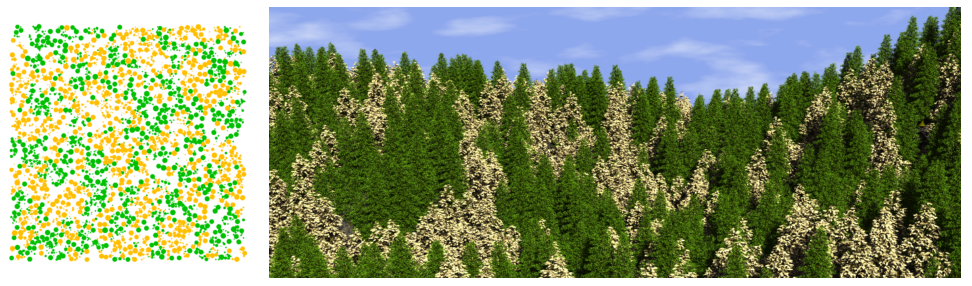
\includegraphics[width=\textwidth]{L-System-Result.png}
    \caption[Plant placement using an ecosystem simulator modelled by L-Systems]{ Plant placement using an ecosystem simulator modelled by L-Systems ~\cite{Lane2002}. \textit{Left:} Result of the simulation where orange circles indicate the positions of poplar trees and green circles the positions of spruce trees. \textit{Right:} Reproduced virtual world where the location of individual plants is deduced from the output of the simulator.}
\end{figure}

Deussen et al. ~\cite{Deussen1998} extend the work by Lane et al. ~\cite{Lane2002} by introducing soil humidity as a constrainer to their L-system based ecosystem simulator.

Probably the main advantage of ecosystem simulators over other approaches is scalability. Running simulations with different species or resource configurations is extremely easy and requires very little input from the user. \\

To run these simulations, however, the user must first configure the properties of the required plant species. These properties (ageing, growth, shade tolerance, humidity preference, etc.) can be hard to obtain.\\
A direct consequence of the ecosystem simulation approach is that fine control over the final vegetative content is lost. Deussen et al. overcome this, however, by offering a hybrid approach where the ecosystem simulator is first used to populate the entire terrain and explicit instancing is used thereafter for the detailing ~\cite{Deussen1998}.\\
The simulation time is proportional to the number of plants present. Therefore, for large or dense areas, the simulation can be computationally intense. \\
Another weakness of procedural ecosystems based on L-Systems worth mentioning is that the communication parameter is binary; in the work by Lane et al. ~\cite{Lane2002} a plant will be dominated as soon as it’s radius intersects another larger plant, at which point it will die with a set probability. This probability of death will stay constant and will not increase as this domination increases. Similarly, in the work by Deussen et al. ~\cite{Deussen1998} when modelling humidity, a plant has a preference for wet or dry areas, there is no notion of a measurable humidity preference.

\todo{CONCLUDE WHICH VEGETATION METHOD WILL BE BROUGHT FORWARD}